%% LyX 1.1 created this file.  For more info, see http://www.lyx.org/.
%% Do not edit unless you really know what you are doing.
\documentclass[10pt,oneside,english,british]{book}
\usepackage{times}
\usepackage[T1]{fontenc}
\usepackage[latin1]{inputenc}
\usepackage{a4wide}
\usepackage{fancyhdr}
\pagestyle{fancy}
\usepackage{babel}
\setcounter{secnumdepth}{3}
\setcounter{tocdepth}{3}
\setlength\parskip{\smallskipamount}
\setlength\parindent{0pt}
\usepackage{graphics}
\IfFileExists{url.sty}{\usepackage{url}}
                      {\newcommand{\url}{\texttt}}

\makeatletter

%%%%%%%%%%%%%%%%%%%%%%%%%%%%%% LyX specific LaTeX commands.
\providecommand{\LyX}{L\kern-.1667em\lower.25em\hbox{Y}\kern-.125emX\@}
%% Special footnote code from the package 'stblftnt.sty'
%% Author: Robin Fairbairns -- Last revised Dec 13 1996
\let\SF@@footnote\footnote
\def\footnote{\ifx\protect\@typeset@protect
    \expandafter\SF@@footnote
  \else
    \expandafter\SF@gobble@opt
  \fi
}
\expandafter\def\csname SF@gobble@opt \endcsname{\@ifnextchar[%]
  \SF@gobble@twobracket
  \@gobble
}
\edef\SF@gobble@opt{\noexpand\protect
  \expandafter\noexpand\csname SF@gobble@opt \endcsname}
\def\SF@gobble@twobracket[#1]#2{}

%%%%%%%%%%%%%%%%%%%%%%%%%%%%%% User specified LaTeX commands.
\renewcommand{\headrulewidth}{0.4pt}
\renewcommand{\footrulewidth}{0.4pt}
\lhead{\resizebox{1in}{!}{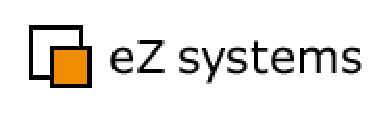
\includegraphics{screenshots/2.0/ezsystems.eps}}}
\rhead{}
\chead{}

\makeatother
\AtBeginDocument{
  \renewcommand{\labelitemiv}{}
}

\begin{document}

\title{eZ publish 2.2 Installation Guide}


\author{\resizebox*{0.75\columnwidth}{!}{
\includegraphics{screenshots/2.0/ezpublish.eps}} }

\maketitle
\resizebox*{!}{0.2in}{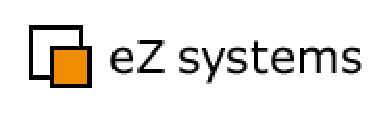
\includegraphics{screenshots/2.0/ezsystems.eps}} The
double squares and eZ are trademarks belonging to eZ systems of Norway,
registration number NO 981 601 564 (http://www.brreg.no/oppslag/enhet/detalj.ssc?orgnr=981601564).

All images and text herein is Copyright 2001 eZ systems.

eZ publish is a software package released under the GPL lisence (http://www.gnu.org/copyleft/gpl.html),
its primary point of distribution and information is http://developer.ez.no/

\tableofcontents{}


\chapter{Introduction\label{chptr: introduction}}

\begin{quote}
\textbf{{}``He who asks is a fool for five minutes, but he who does
not ask remains a fool forever.''} - \- Chinese proverb
\end{quote}
eZ publish is a content management system, among a lot of other things.
This installation manual will try to cover the job of installing eZ
publish on your server.

Since version 2.2 eZ publish has a new possible way to be installed:
without virtual hosts and mod\_rewrite. This makes it possible for
people, who don't have a dedicated server or a specialized eZ publish
hoster, to install eZ publish on their accounts as long as they have
PHP and a supported database (e.g. mySQL or PostgreSQL). 

This opens some new options for installing:

If you have an account at a webhoster with PHP and mySQL, your option
should be chapter \ref{chpt: nVH}, because you won't be able to install
eZ publish as it's explained in chapter \ref{chpt: dedicated server}.

If you have a dedicated server with Apache and mySQL already running
and you don't want to mess with the Apache configuration, then chapter
\ref{chpt: nVH} might be of interest of you. 

If you have a dedicated server and want some help on how to install
all needed software and eZ publish on it, then chapter \ref{chpt: dedicated server}
is for you.


\section{Pre-Configured Hosting}

It is possible to get pre-configured hosting services where you can
install and manage your eZ publish site with ease. Read more about
our hosting partners at eZ systems web site (\texttt{\footnotesize http://}ez.no/shop/hosting).


\section{Pre-Configured Hardware}

It is possible to order pre-configured hardware from eZ systems. You
can order through or web shop (\texttt{\footnotesize http://}shop.ez.no).

A line starting with a hash-sign {}``\#'' are input from the user
to the shell.


\chapter{\label{chpt: dedicated server}Installing eZ publish (standard\footnote{%
An alternative install method is described in chapter \ref{chpt: nVH}
} method)}

This chapter is mainly intended for installation on a Red Hat Linux
system, but a lot of friendly people have contributed information
for installation on other operating systems, take a look at chapter
2 and learn which systems those are.

Most of what is described here regarding Red Hat installation can
also be applied to other installations, especially if your system
uses RPM for installation. For other systems you would need to do
a lot of compiling yourself to make this work, or apply the system's
own package manager.

Finding packages can be done dirctly from vendor sites, though you
might not be guaranteed that you'll find the package you need. In
such instances you need to download the source directly from the software
developer.

Different distribution sites for different Unix systems are:

\begin{itemize}
\item Debian \texttt{\footnotesize (http://www.debian.org/distrib/ftplist)}{\footnotesize \par}
\item Mandrake, see chapter \ref{chptr: mandrake}.
\item IRIX \texttt{\footnotesize (http://freeware.sgi.com/)}{\footnotesize \par}
\item Red Hat Linux \texttt{\footnotesize (http://www.redhat.com/apps/download})
\item SuSE Linux (\texttt{\footnotesize http://www.suse.com/us/support/download/index.html)}{\footnotesize \par}
\item Sun \texttt{\footnotesize (http://www.sunfreeware.com/)}{\footnotesize \par}
\end{itemize}
The addresses to the software developers will be given where appropriated
in the text.

You can also try \char`\"{}The Written Word\char`\"{} (\texttt{\footnotesize ftp://ftp.thewrittenword.com/packages/free/by-name/gcc-2.95.2/})
for binaries for Solaris 2.5.1, 2.6, 2.7/SPARC, 2.7/Intel, IRIX 6.2,
6.5, Digital UNIX 4.0D, HP-UX 10.20, and HP-UX.


\section{Prerequisites\label{chptr: pre-requisites}}


\subsection{Needed Privileges}

For the standard installation of eZ publish you will need to have
the following privileges on your system:

\begin{itemize}
\item Access to Apache's httpd.conf for creating two virtual hosts and for
enabling the rewrite engine and creating rewrite rules. This is absolutely
necessary for eZ Publish at the moment.
\item Access to compiler, only needed if you can't use any of the pre-compiled
packages available. (You will have to install the gcc compiler on
your system, see chapter \ref{chptr: introduction} for a list of
sites providing software for different Unixes.)
\item Access to a shell (You must run certain scripts during installation,
and sometimes for maintenance.)
\item Access to cron jobs (Only needed if you want to use the eZ news feed
module for regular updates of headlines imported from other sites.)
\item Access to Apache's modules
\item Access to a MySQL or PostgreSQL database
\item You might also need the privilege to add new libraries to your system.
\end{itemize}
You might also use other web servers than apache, but then you're
on your own since we haven't tested eZ publish on other configurations.
If you do try another web server, please keep a log of what you do
and submit it to us (pkej@ez.no) for inclusion in future versions
of this manual.


\subsection{Needed Software}

You also need to download and install the following packages, if they
aren't present on your system already:

\begin{itemize}
\item A database. Currently, eZ publish suppports MySQL (http://www.mysql.com)
version 3.23 or later and PostgreSQL (http://www.postgresql.org) version
7.1.3 or later.
\item ImageMagick (http://www.imagemagick.org/) newest version (Needed by
eZ article, eZ image catalogue, and all modules using images. You
need only the command line version.)
\item Apache (http://httpd.apache.org/) latest 1.3 release. (It is always
recommended to run the latest Apache release, though eZ publish shouldn't
be very picky with the Apache versions. We've used eZ publish with
Apache 1.3.13, some have reported that Apache 1.3.9 isn't useful.)
\item mod\_rewrite. This apache module is included in all recent versions
of RedHat Linux. If you use an other distro, you may need to recompile
apache with mod\_rewrite
\item Any and all modules you need for apache in addition to mod\_php. (http://modules.apache.org/)
\item PHP (http://www.php.net/) version 4.0.4pl1 or later. Version 4.0.6
is recommended. You need the source code version from this site, for
windows you can just download the binary. (eZ publish uses references
for objects and foreach loops. Only version 4.0.4pl1 and later supports
both of these features satisfactorily.)
\item eZ publish (http://developer.ez.no/) verision 2.0 or later stable
releases.
\end{itemize}
The libraries and php are packaged pre-compiled for Linux i386 on
http://developer.ez.no. The software is listed in the order of installation.

You should also find a list of RPMs at http://www.brandish.co.uk/phprpm

\textbf{Important release note:}

eZ publish version 2.2.2 does not require neither QDom or libxml as
previosly releases did. In this release, eZ publish uses it own xml
parser : eZ xml. Optioninal support for libxml will probably be reintroduced
in a future version of eZ publish


\subsection{Which Software is Already Installed?}


\subsubsection{Systems Using RPM}

RPM is a system for distributing pre-compiled software. The packages
also contain pre-configured settings and initialisation files, leaving
almost nothing to the user, except deciding what to install.

To check if a package is available on your system you can run the
following command (RPM based systems {}``rpm -qa | grep <name of
program/library>''. If you need to know where you can find the different
files from that package you can follow up on the previous command
with the following {}``rpm -ql <rpm name>''. RPM name is one of
the returned names from the previous command, example\footnote{%
A line starting with a hash-sign \char`\"{}\#\char`\"{} are input
from the user to the shell.
}:\\


\texttt{\footnotesize ~~~~\# rpm -qa | grep libxml}{\footnotesize \par}

\texttt{\footnotesize ~~~~libxml-1.8.7-80}{\footnotesize \par}

\texttt{\footnotesize ~~~~libxmld-1.8.7-80}{\footnotesize \par}

\texttt{\footnotesize ~~~~\# rpm -ql libxml-1.8.7-80}{\footnotesize \par}

\texttt{\footnotesize ~~~~/usr/bin/xml-config}{\footnotesize \par}

\texttt{\footnotesize ~~~~/usr/lib/libxml.so.1}{\footnotesize \par}

\texttt{\footnotesize ~~~~/usr/lib/libxml.so.1.8.7}{\footnotesize \par}

\texttt{\footnotesize ~~~~/usr/share/doc/packages/libxml}{\footnotesize \par}

\texttt{\footnotesize ~~~~/usr/share/doc/packages/libxml/AUTHORS}{\footnotesize \par}

\texttt{\footnotesize ~~~~/usr/share/doc/packages/libxml/COPYING}{\footnotesize \par}

\texttt{\footnotesize ~~~~/usr/share/doc/packages/libxml/COPYING.LIB}{\footnotesize \par}

\texttt{\footnotesize ~~~~/usr/share/doc/packages/libxml/NEWS}{\footnotesize \par}

\texttt{\footnotesize ~~~~/usr/share/doc/packages/libxml/README}{\footnotesize \par}

\texttt{\footnotesize ~~~~/usr/share/doc/packages/libxml/TODO}{\footnotesize \par}


\subsection{Mandrake}

First read chapter \ref{chptr: mandrake}, then continue reading the
manual from here.


\subsection{IRIX}

By accessing the software manager (you must be root) you can get a
list of installed software, scroll or search that list to find the
packages you're interested in. Double click on the tabs to the left
to get information about where specific files are installed.


\subsection{RAQ 3}

There is a separate chapter \ref{chptr: raq 3} in this manual describing
installation on a RAQ 3 server. It was kindly provided by Chris Mason, 


\subsection{Windows}

Windows installation is described in its own chapter \ref{chptr: windows}.


\subsection{Other Systems}

On other systems you should read the documentation for that system
to learn how to find out what software is already installed.

You could try to use the command {}``find'' to find the software.
It is used thus: {}``find . -name \textbackslash{}{*}<program name>\textbackslash{}{*}''
from the /usr/, /local/ , /lib/, /share/ directories. In extreme cases
you could try from the root of the system, but this will take a long
time and will also hog resources on your computer. Therefore we urge
you to learn how to use the proper installation features of your system
to find the software already installed.


\subsection{Installation of Required Software}

If you've found pre-compiled versions of all the software packaged
for use with an installation tool, you just have to install that software
using the tool. Instructioins for its usage is often found using the
command {}``man <installation tool name>'' or by reading your system's
documentation or the supplier's website.

If you've had to download source code you will find instructions on
how to compile and install the software you've downloaded at the software
developer's website. This requires a bit of knowledge and you should
only undertake this if you feel confident about the job.

This manual will only cover configuration of the software needed and
compilation of PHP to use the other software.


\subsection{Important Notice}

You should read all the README, INSTALL and similar files found with
the software packages you download. They often contain tips on how
to configure, compile and install the software on your system. It
will save you a lot of time and aggravation if you follow instructions
supplied with the software.

If problems arise during installation of the software, please turn
to the suppliers support forums, mailing list archives and FAQs, your
questions will often be answered there. If the supplier's forums doesn't
seem to help you, you should check the support forums at our site.

You should always do a search of the forums before posting any questions.


\section{Compile Configuration}


\subsection{PHP}

Important : YOU NEED TO RECOMPILE PHP. No known Linux distros does
yet have all the php features required by eZ~publish. This means
that you need to compile the php module from source.\\
You may find precompiled binaries for your system at the eZ publish web site,  \url{http://developer.ez.no}.
Take a look at the {}``Contributions'' section in the download area.


\subsubsection{Unpacking}

After you have downloaded PHP you need to unpack it somewhere where
you can compile and configure the software. To unpack run the command:\\


\texttt{\footnotesize ~~~~\# tar zxvf php-4.0.x.tar.gz}~\\
{\footnotesize \par}

Where the x is the version of php you've downloaded. Then you need
to move into the directory you extracted php into:\\


\texttt{\footnotesize ~~~~\# cd php-4.0.x}{\footnotesize \par}


\subsubsection{Configuration}

You'll need either an apache module or a command line (CGI) version
of PHP to use eZ publish on your website. We recommend you use PHP
as an apache module. You will also need the command line version if
you want to use the cron jobs for periodical updates of the eZ news
feed module.

Thus for our recommended installation of PHP you need both the command
line and module versions of PHP.


\paragraph{Common}

Both the command line and apache module versions need to have the
following configurations added to the configuration tool:

\begin{description}
\item [--enable-trans-sid]This lets PHP use session id's which don't rely
on cookies. It does not disable normal cookie based sessions.\\
({\footnotesize http://www.php.net/manual/en/install.configure.php\#install.configure.enable-trans-sid})
\item [--with-mysql]This tells PHP that the mysql functionality should be
used.\\
({\footnotesize http://www.php.net/manual/en/install.configure.php\#install.configure.with-mysql})
\item [--disable-magic-quotes]This tells PHP to disable magic quotes by
default. you can also turn this feature on and off on a directory
by directory basis in either the {}``.htaccess'' files (if you use
them) or in the setup of the virtual server in {}``httpd.conf''.
\item [IMORTANT]: From version 2.1\footnote{%
eZ publish versions prior to 2.1 required magic quotes to be enabled
} onwards magic quotes must be turned off for eZ publish to work properly.\\
({\footnotesize http://www.php.net/manual/en/install.configure.php\#install.configure.enable-magic-quotes})
\item [--with-imap]This configures PHP to include imap support. This is
used by eZ mail module. This parameters require ssl support. Imap
does also have bindings to kerberos. This causes some linking problems
on RedHat Linux. The workaround for this problem is to type this command
before you compile : \texttt{\footnotesize }~\\
\texttt{\footnotesize }~\\
\texttt{\footnotesize \$ export LDFLAGS=\char`\"{}-L/usr/kerberos/lib
-lkrb5 -lgssapi\_krb5~-lpam\char`\"{}}{\footnotesize \par}
\item [--with-openssl]This will enable ssl support in PHP
\end{description}
You should also go through the web page: {\footnotesize http://www.php.net/manual/en/install.configure.php}
and make sure that there isn't other functionality you would like
to have included.


\paragraph{Command Line}

The default is to create a command line version of PHP. Therefore
you don't need to add more configuration options for this.


\paragraph{Apache Module}

To build an apache module you need to add:

\begin{description}
\item [--with-apxs]This compiles PHP as an apache module. {\footnotesize }\\
{\footnotesize (http://www.php.net/manual/en/install.configure.php\#install.configure.with-apxs)}{\footnotesize \par}
\end{description}

\paragraph*{Other Web Servers}

We haven't tested our software with other web servers than apache.
If you need to try out other web servers, read this document {\footnotesize http://www.php.net/manual/en/install.configure.php\#install.configure.servers}
to learn how you configure for the web server you will be using.


\paragraph{Creating the Configuration}

Now you just have to run the {}``./configure'' program with the
appropriate configuration directives which we discussed in the preceeding
sections, for an apache module you'd do the following:\\


\texttt{\footnotesize ~~~\# ./configure -{}-enable-trans-sid -{}-with-mysql
-{}-enable-trans-sid -{}-disable-magic-quotes -{}-with-imap -{}-with-openssl}~\\
\texttt{\footnotesize ~~~~-{}-with-apxs}~\\
{\footnotesize \par}

Remember that to compile a script/cgi version you'd need to change
that line to:\\


\texttt{\footnotesize ~~~~\# ./configure -{}-enable-trans-sid
-{}-with-mysql -{}-enable-trans-sid -{}-disable-magic-quotes -{}-with-imap
-{}-with-openssl}~\\
\texttt{\footnotesize ~~~~}{\footnotesize \par}


\subsubsection{Compilation}

To compile you need to run the command {}``make'':\\


\texttt{\footnotesize ~~~~\# make}{\footnotesize \par}


\subsubsection{Installation}

To install your new PHP package you need to run the following command:\\


\texttt{\footnotesize ~~~~\# make install}{\footnotesize \par}


\subsubsection{Compiling the php module on RedHat 7.x, step by step}

First download the source from www.php.net. You should get a file
called something like

php-4.0.6.tar.gz\\


First, unpack the tarball:

\texttt{\footnotesize \$ tar -xzf php-4.0.6.tar.gz}\\


Now, enter the source directory

\texttt{\footnotesize \$ cd php-4.0.6}\\


Apply the kerberos workaround:

\texttt{\footnotesize \$ export LDFLAGS=\char`\"{}-L/usr/kerberos/lib
-lkrb5 -lgssapi\_krb5 -lpam\char`\"{}}\\


Run the configure script:

\texttt{\footnotesize \$ ./configure -{}-with-apxs=/usr/sbin/apxs
-{}-enable-ftp -{}-enable-trans-sid -{}-with-config-file-path=/etc/httpd
-{}-with-mysql=/usr -{}-with-pgsql=/usr -{}-enable-inline-optimization
-{}-with-ttf -{}-with-gd -{}-enable-gd-native-ttf -{}-with-imap -{}-includedir=/usr
-{}-with-openssl=/usr -{}-with-zlib-dir=/usr -{}-with-openssl=shared,/usr}~\\
{\footnotesize \par}

Compile the module:

\texttt{\footnotesize \$ make}\\


Install the module, either automaticly or manually.\\
Manually : 

\texttt{\footnotesize \$ su}{\footnotesize \par}

\texttt{\footnotesize \# cp .libs/libphp.so /usr/lib/apache}{\footnotesize \par}

Automaticly:

\texttt{\footnotesize \$ su}{\footnotesize \par}

\texttt{\footnotesize \# make install}\\


Restart apache:

\texttt{\footnotesize \# /etc/rc.d/init.d/httpd restart}\\


Verify that everything went OK.\\
Verify that apache was able to start:

\texttt{\footnotesize \# ps ax | grep httpd}\\


Check the apache log

\texttt{\footnotesize \# tail -f 50 /var/log/httpd/error\_log}~\\
{\footnotesize \par}

IMPORTANT

When compiling php, please read chapter \ref{chptr: Troubleshooting}.
Especially, take note of chapter \ref{chptr: openssl problem on redhat}.
It might save you for hours with debugging


\section{Apache Configuration}

If you don't want to change the Apache configuration, go to chapter
2. Please take notice of the rewrite rules. They have been changed
since the previously versions.


\subsection{Dual Virtual Host\label{sec: dual virtualhost}}


\subsubsection{Configuring Through httpd.conf}

This set up is based on having two different virtual hosts for your
administration back-end and the main site. The main site would typically
be known as {}``www.yoursite.com'' and the administration would
be {}``admin.yoursite.com''; the names are up to you, theoretically
you could have different names, for example {}``mysite.yoursite.com''
and {}``administration.mysite.com''.

The virtual host is configured through the {}``httpd.conf'' file
which is the main configuration of Apache. Following is an example
of such a host, modify it to reflect your own installation and preferences,
but before that be sure to add the {}``NameVirtualServer'' directive
to the configuration file. The directive is {}``NameVirtualServer
ip-address'' where the ip address is the address where the server
will receive requests (http://httpd.apache.org/docs/mod/core.html\#namevirtualhost).

You should consider using the utility which we have online for creating
the configuration. The URL is http://developer.ez.no/virtualhost it
will generate a setup with the latest needed information. The presented
configuration herein might be slightly outdated, so we recommend the
online tool.


\paragraph{User Site}

\texttt{\scriptsize ~~~~\# User site}{\scriptsize \par}

\texttt{\scriptsize ~~~~<VirtualHost~your.ip.addr.no>}{\scriptsize \par}

\texttt{\scriptsize ~~~~~~<Directory /your/docroot>}{\scriptsize \par}

\texttt{\scriptsize ~~~~~~~~Options FollowSymLinks}{\scriptsize \par}

\texttt{\scriptsize ~~~~~~~~AllowOverride None }{\scriptsize \par}

\texttt{\scriptsize ~~~~~~</Directory>}{\scriptsize \par}

\texttt{\scriptsize ~~~~~~RewriteEngine On}{\scriptsize \par}

\texttt{\scriptsize ~~~~~RewriteRule .{*}/ezmediacatalogue/catalogue/(.{*})\$
/your/docroot/ezmediacatalogue/catalogue/\$1 {[}T=\char`\"{}application/oct-stream\char`\"{},S=4{]}}{\scriptsize \par}

\texttt{\scriptsize ~~~~~~RewriteRule \textasciicircum{}/stats/store/(.{*}).gif\$~
/your/docroot/ezstats/user/storestats.php {[}S=3{]}}{\scriptsize \par}

\texttt{\scriptsize ~~~~~~RewriteRule \textasciicircum{}/filemanager/filedownload/({[}\textasciicircum{}/{]}+)/(.{*})\$~
/your/docroot/ezfilemanager/files/\$1 {[}T=\char`\"{}application/oct-stream\char`\"{},S=2{]}}{\scriptsize \par}

\texttt{\scriptsize ~~~~~~RewriteRule \textasciicircum{}/mediacatalogue/catalogue/(.{*})\$~
/your/docroot/ezmediacatalogue/catalogue/\$1 {[}T=\char`\"{}application/oct-stream\char`\"{},S=1{]}}{\scriptsize \par}

\texttt{\scriptsize ~~~~~~RewriteRule !\textbackslash{}.(gif|css|jpg|png|jar)\$
/your/docroot/index.php}{\scriptsize \par}

\texttt{\scriptsize ~~~~~~ServerAdmin your.e-mail@address}{\scriptsize \par}

\texttt{\scriptsize ~~~~~~DocumentRoot /your/apache/documentroot/publish\_dist}{\scriptsize \par}

\texttt{\scriptsize ~~~~~~ServerName your.domain.com}{\scriptsize \par}

\texttt{\scriptsize ~~~~</VirtualHost>}{\scriptsize \par}


\paragraph{Admin Site}

\texttt{\footnotesize ~~\# Admin site }{\footnotesize \par}

\texttt{\footnotesize ~~<VirtualHost your.ip.addr.no>}{\footnotesize \par}

\texttt{\footnotesize ~~~~}\texttt{\scriptsize <Directory /your/docroot>}{\scriptsize \par}

\texttt{\scriptsize ~~~~~~~ Options FollowSymLinks}{\scriptsize \par}

\texttt{\scriptsize ~~~~~~~ AllowOverride None }{\scriptsize \par}

\texttt{\footnotesize ~~~~}\texttt{\scriptsize </Directory>}{\scriptsize \par}

\texttt{\footnotesize ~~~~}\texttt{\scriptsize RewriteEngine On}{\scriptsize \par}

\texttt{\scriptsize ~~~~RewriteRule .{*}/ezmediacatalogue/catalogue/(.{*})\$
/your/docroot/ezmediacatalogue/catalogue/\$1 {[}T=\char`\"{}application/oct-stream\char`\"{},S=1{]}}{\scriptsize \par}

\texttt{\footnotesize ~~~~}\texttt{\scriptsize RewriteRule !\textbackslash{}.(gif|css|jpg|png|jar)
/your/docroot/index\_admin.php}{\scriptsize \par}

\texttt{\footnotesize ~~~~ServerAdmin your\_mail@domain.no}{\footnotesize \par}

\texttt{\footnotesize ~~~~DocumentRoot /your/apache/documentroot/publish\_dist}{\footnotesize \par}

\texttt{\footnotesize ~~~~ServerName admin.yourdomain.org}{\footnotesize \par}

\texttt{\footnotesize ~~</VirtualHost>}~\\
{\footnotesize \par}

The format of the {}``httpd.conf'' file is covered at http://httpd.apache.org/docs/
for a complete understanding of the above information you'll need
to read that documentation.

The directory {}``/your/docroot/'' is the directory where you extracted
eZ publish.


\paragraph{Error Checking}

You can check that everything is correct with your rewrite rules by
running {}``apache -s'', which will check for virtual hosts. There
should also be an error log (consult the apache documentation) which
you can read to check for errors.


\paragraph{Explanation of the Rewrite Rules}

A rewrite rule contains three arguments. The third argument is optional.
The first argument describes a (reg exp\footnote{%
For an introduction to regular expressions, take a look at http://zez.org/article/articleview/11/
}) pattern which is applied to the URI. If the URI match the regular
expression, the URI is substituted with the second argument . A last
argument can be used to give mod\_rewrite special flags so that it's
behaviour will differ from the default. The syntax for a rewrite rule
can be written in this general form:

\texttt{\footnotesize ~~~~~RewriteRule Pattern Substitution {[}FLAGS{]}}\\


The rewrite rules for eZ publish do the following:\\
\\
\texttt{\footnotesize ~~~~~RewriteRule .{*}/ezmediacatalogue/catalogue/(.{*})\$
/your/docroot/ezmediacatalogue/catalogue/\$1 {[}T=\char`\"{}application/oct-stream\char`\"{},S=4{]}}{\footnotesize \par}

This rewrite rule states that every URLs containing the string {}``\texttt{\footnotesize /ezmediacatalogue/catalogue/}''
shall be served from {}``\texttt{\footnotesize /your/docroot/ezmediacatalogue/catalogue/}''.
The {}``\texttt{\footnotesize .{*}}'' means zero or more characters
of any type. When this is written in parenthesis like at the end of
the argument, these characters in inserted in the variable \$1. The
result of this is that the filename is inserted into the variable
\$1. The trailing \$ in the pattern argument is a special meaning
in a regular expression. It is the a symbol for the end of the line.
In the substitution argument, the content of variable \$1 is then
appended to the path {}``\texttt{\footnotesize /your/docroot/ezmediacatalogue/catalogue/}''
so that the correct file is served.\\
An result of this rewrite rule is that a file in the mediacatalog
will be served independet if which user is logget on. Permissions
on the media file will not checked if the user knows the filename.
This will be fixed in a later version of eZ publish.\\


\texttt{\scriptsize ~~~~~~RewriteRule \textasciicircum{}/stats/store/(.{*}).gif\$~
/your/docroot/ezstats/user/storestats.php {[}S=3{]}}~\\
{\scriptsize \par}

This says that everything served from {}``/stats/store/'' should
be served by the storestats.php script. This is used by the statistical
module

\texttt{\scriptsize ~~~~~~RewriteRule \textasciicircum{}/filemanager/filedownload/({[}\textasciicircum{}/{]}+)/(.{*})\$~
/your/docroot/ezfilemanager/files/\$1 {[}T=\char`\"{}application/oct-stream\char`\"{},S=2{]}}~\\
{\scriptsize \par}

This says that everything served from {}``/filemanager/filedownload/''
should be redirected to fetch information from {}``publish\_dist/ezfilemanager/files''.
In other words, when people downloads a file from the filemanager,
the file is served from the directory specified in the second part.

The {}``\^{ }'' just after {}``RewriteRule'' says that evertything
which starts with this, in other words it is a start of line marker.
When working with an URL that is from the root of your site, ie. the
part from the first slash after your domain name.

The {}``\$'' sign is used to mark the end of line, in order to remember
the full line.

The part \texttt{\scriptsize {}``{[}T=\char`\"{}application/oct-stream\char`\"{},S=2{]}''}
means that everything which is matched shall be of the specific mime
type ({}``application/oct-stream'', ie. binary download). The {}``S=1''
part means that if we match this rule, we should skip one rule ahead
before trying to match again.\\


The last rewrite rule

\texttt{\scriptsize ~~~~~~RewriteRule !\textbackslash{}.(gif|css|jpg|png|jar)\$
/your/docroot/index.php}~\\
{\scriptsize \par}

is found in both sites (admin and user). This means that every file,
except gif, css, jpg and png (and files matched against the previous
rule when in the user site) should be redirected to the file in the
second part, ie. the index.php or index\_admin.php file. The reason
for this is that we don't want anyone trying to get direct access
to anything which might be sensitive, or revealing about the site's
operation.

If you compiled PHP with magic quotes; or other software relies on
PHP using magic quotes you can add the following line into each virtual
host section:\\


\texttt{\footnotesize ~~~~php\_flag magic\_quotes\_gpc off}{\footnotesize \par}

\texttt{\footnotesize ~~~~php\_flag magic\_quotes\_runtime off}~\\
{\footnotesize \par}


\subsubsection{Configuring php.ini}

Magic quotes may also be turned of in php. This will disable magic
quotes:

\texttt{\scriptsize magic\_quotes\_gpc = Off}{\scriptsize \par}

\texttt{\scriptsize magic\_quotes\_runtime= Off}{\scriptsize \par}


\subsubsection{Configuring Through .htaccess}

At present, configuring the rewrite rules in .htaccess files is not
supported. However, you may switch of magic quotes in an .htaccess
file.

\emph{Note: You must set up apache to accept this.}


\paragraph{User Site}

In your document root (/path/to/index.php/) create a file called \char`\"{}.htaccess\char`\"{}
containing the following text:\\


\texttt{\footnotesize ~~~~php\_flag magic\_quotes\_gpc off}{\footnotesize \par}


\section{eZ publish Installation}


\subsection{Program Files}

The next step is to install the eZ publish package in your document
root directory. First you need to unpack the software in a temporary
directory:\\


\texttt{\footnotesize ~~~~\# cd /tmp}{\footnotesize \par}

\texttt{\footnotesize ~~~~\# tar zxvf /path/to/ezpublish-2.0.tar.gz}~\\
{\footnotesize \par}

The next step is to move the files to your document root:\\


\texttt{\footnotesize ~~~~\# mv /tmp/publish\_dist /your/apache/documentroot}~\\
{\footnotesize \par}

When all this is done you need to tell eZ publish a little about the
site you're running. You'll need to edit the {}``site.ini'' file
which you will find in the document root:\\


\texttt{\footnotesize ~~~~\# cd /your/apache/documentroot}{\footnotesize \par}

\texttt{\footnotesize ~~~~\# vi site.ini}~\\
{\footnotesize \par}

Instead of vi you can use your preferred text editor. You'll need
to add information about the username, hostname and password of your
database. More information on what you can do with {}``site.ini''
can be found in the {}``eZ publish Customisation Guide''.

The next important step is to run the script {}``modfix.sh''. \\


\texttt{\footnotesize ~~~~\# ./modfix.sh}~\\
{\footnotesize \par}


\subsection{\label{sec: Database (dual hosts)}Database }

Some people might prefer to use phpMyAdmin (http://www.phpwizard.net/projects/phpMyAdmin/)
for most of this part; we can not help you with installation of that
program, though.


\subsubsection{First time installation (MySQL)}

Now you need to create a database in MySQL, the default name we use
is publish, but you can change that to whatever pleases you.\\


\texttt{\footnotesize ~~~~\# mysqladmin create publish}~\\
{\footnotesize \par}

Add a publish user in MySQL. To add a user you can use the MySQL client
to log on to mysql and then create the user:\\


\texttt{\footnotesize ~~~~\# mysql > grant all on publish.{*}
to publish@localhost}{\footnotesize \par}

\texttt{\footnotesize ~~~~identified by \char`\"{}secret\char`\"{};}\texttt{}~\\


where secret is your password. Then you need to add the default eZ
publish data into your newly created database:\\


\texttt{\footnotesize ~~~~\# mysql -uroot -p publish < sql/publish\_mysql.sql}{\footnotesize \par}


\paragraph{Adding Pre-Defined Data}

If you want to add the pre-defined data of the distribution you shouldn't
add any data manually to the site before executing these commands.

First we need to add files and images which are needed by the database.\\


\texttt{\footnotesize ~~~~\# tar zpxvf data.tar.gz}~\\
{\footnotesize \par}

Then we need to run {}``modfix.sh'' to make sure that everything
is readable.\\


\texttt{\footnotesize ~~~~\# ./modfix.sh}~\\
{\footnotesize \par}

Then we need to send the SQL data into the database:\\


\texttt{\footnotesize ~~~~\# mysql -upublish -ppublish publish
< sql/data\_mysql.sql}~\\
{\footnotesize \par}

Finally we run clearcache\footnote{%
A new feature in eZ publish 2.2 is the possibility of clearing the
cache from the admin site
} to make sure that everything presented is cached correctly:\\


\texttt{\footnotesize ~~~~\# ./clearcache.sh}{\footnotesize \par}


\subsubsection{PostgreSQL configuration}

Important note regarding PostgreSQL support in eZ publish:

PostgreSQL has one limitation which is not good for eZ publish:

Max length of indentifiers used in the database, table names, column
names etc is default set to 32.

eZ publish uses names which sometimes are longer, e.g: eZImageCatalogue\_ImageVariationGroup

Therefore you need to recompile PostgreSQL to support a larger value
by altering: 

\begin{verse}
\#define NAMEDATALEN 64
\end{verse}
in the file : src/include/postgres\_ext.h


\subsubsection{PostgreSQL setup}

On last configuration change is necessary. This will allow TCP-IP
connections to the database, not only unix sockets. 

In pqsql-root/data/postmaster.opts (for instance /var/lib/pgsql/data/postmaster.opts)
you need to apply a {}``-i'' parameter. The content of the file
will then be like this:

\texttt{\scriptsize /usr/bin/postmaster '-D' '/var/lib/pgsql/data/'
'-i'}{\scriptsize \par}


\subsubsection{First time installation (PostgreSQL)}

Login as user postgres

\texttt{\footnotesize ~~~~\# su - postgres}~\\
{\footnotesize \par}

Create a database

\texttt{\footnotesize ~~~~\$ createdb publish}~\\
{\footnotesize \par}

Create a dabase user

\texttt{\footnotesize ~~~~\$ createuser publish -W}~\\
{\footnotesize \par}

Create tables

\texttt{\footnotesize ~~~~\$ psql -Upublish <sql/data\_mysql.sql}~\\
{\footnotesize \par}

You also need to enable PostgreSQL in site.ini. Change the'' DatabaseImplementation''
configuration so it reads:

\begin{verse}
DatabaseImplementation=postgresql
\end{verse}

\subsubsection{Updating the Installation}

This section is for users who are updating from a previous version
of eZ publish. There should be several files ending with {}``.sql''
in the directory {}``updates''. Run the files needed to update your
version to the current. You need to apply all the updates for every
version since your version.


\section{Now What?}

After installing eZ publish you can test your site through the URL
\texttt{\footnotesize http://www.yoursite.com/} and you can administrate
your site from the URL \texttt{\footnotesize http://admin.yoursite.com/},
of course, if you did anything different the names of the admin and
the public site might be different.

\emph{NOTE:} The default user name and password for your site will
be admin/publish. Remember to change the password.

The next manual you should read is the {}``eZ publish Customisation
Guide'', it tells you how to configure the software to use the functionality
you want, as well as how you change the templates to suit your needs.

When you're finished with the design and the initial testing you can
head over to \texttt{\footnotesize http://zez.org/} for articles about
community building as well as programming, or you can visit \texttt{\footnotesize http://developer.ez.no}
for updates, articles about eZ publish and how to work with it, as
well as keeping abreast of new developments.


\subsection{Post Install Checklist}

\begin{enumerate}
\item Does Apache run?
\item Does PHP run/work as an Apache module?
\item Does MySQL run?
\item Can you access your virtual hosts at all?
\item Does the user site work?
\item Does the admin site work?
\item Consider this: all eZ publish sites has an admin site, perhaps you
should call the admin host something different than admin?
\item Check that you've downloaded and read the configuration manual. A
quick tip is to read through the file {}``site.ini'' and change
any e-mail addresses, passwords etc. to fit your own choices.
\item Log in on your admin site (\texttt{\footnotesize http://admin.yoursite.com/}).
You will be presented with a page which will list any install problems.
If any problems appear read the error message presented and follow
any instructions. If that fails, read the FAQ. Then go to \texttt{\footnotesize http://developer.ez.no}
and search the forum for anyone who have had the same problem. Also
check the bug list for any open bugs covering your problem. Finally
you should register to the mailing list and try asking for help there.
\item If everything is okay go to the {}``user'' module and change the
e-mail address of the site administrator immediatly.
\item Change the password of the administration user to something only you
know.
\item Start browsing the public part of your site, just to check that everything
is working; some of the articles supplied as default will inform you
about features of the software.
\item Check that ImageMagick is working. Try to upload an image to your
site.
\end{enumerate}

\section{\label{chptr: Troubleshooting}Troubleshooting}


\subsection{Problems During Installation}


\subsubsection{Missing Compiler/Can not Compile (C++/C)}

When compiling php and other support programs (like ImageMagick) you
need the GCC compiler. It is recommended that you use the GCC compiler
which was shipped with your Linux distro/unix system. In the introduction
(see chapter \ref{chptr: introduction}) it listed some sites where
you can download pre-compiled versions of software for some different
Unix versions. Please note that you must compile php on your own.


\subsubsection{I am getting linking errors when trying to build PHP}

The PHP module you have compiled will be linked agains kerberos. This
causes some linking problems on RedHat Linux. The workaround for this
problem is to type this command before you compile :

\texttt{\footnotesize \$ export LDFLAGS=\char`\"{}-L/usr/kerberos/lib
-lkrb5 -lgssapi\_krb5 -lpam\char`\"{}}{\footnotesize \par}


\subsection{Problems After Installation}


\subsubsection{Permission Denied}

\texttt{\small Warning: fopen(\char`\"{}site.ini\char`\"{},\char`\"{}r+\char`\"{})}{\small \par}

\texttt{\small Permission denied in classes/INIFile.php on line 80}{\small \par}

If you get this error message you need to run the {}``modfix.sh''
script.


\subsubsection{Can not see Images}

ImageMagick is not working, make sure that it is working by using
the command line command {}``convert''.


\subsubsection{Warning about Temp Directory}

If you get any such warning you need to set the temp directory in
php.ini.


\subsubsection{\label{chptr: openssl problem on redhat}After installing my new
php module, apache dies immediately.}

RedHat as released new versions of the openssl packages for RedHat
7.x\footnote{%
The problem described here may only apply to RedHat 7.0
}. If these erratas is installed before you compile php, your php module
will be linked agains these. This will however brake mod\_ssl, which
is linked to the old openssl libraries. There are two different ways
to fix this:\\
Uninstall mod\_ssl:

\# rpm -e mod\_ssl\\
\\
Or you may download the apache source rpm from redhat. Then recompile
and install it.\\


If this doesn't help, look for clues in /var/log/httpd/error\_messages


\section{Installing on RAQ 3\label{chptr: raq 3}}

\emph{Installing ezPublish on raq3 without messing up the GUI or voiding
the warranty.}

This is untested by eZ systems, and we provide this {}``as is''
without any form of guarantee or endorsement, either explicitly or
implicitly.

First, add the domain into the DNS, but do not create a virtual site.

Log in by telnet (install SSH unless you are desperate to get hacked).

Put the publish files in the directory you want to use, I used /home/sites/extrasites/mysite/web

Install mysql 3.23 or later by rpm, there is one out there. MySQL
(http://www.mysql.com) version 3.23 or later if you want to compile

Now you need to create a database in MySQL, the default name we use
is publish, but you can change that to whatever pleases you.\\


\texttt{\footnotesize ~~~~\# mysql -uroot -p publish < sql/publish.sql}~\\
{\footnotesize \par}

Add a publish user in MySQL. To add a user you can use the MySQL client
to log on to mysql and then create the user:\\


\texttt{\footnotesize ~~~~\# mysql>grant all on publish.{*} to
publish@localhost}{\footnotesize \par}

\texttt{\footnotesize ~~~~identified by \char`\"{}secret\char`\"{};}~\\
{\footnotesize \par}

where secret is your password. Then you need to add the default eZ
publish data into your newly created database:\\


\texttt{\footnotesize ~~~~\# mysql -uroot -p publish < sql/publish.sql}~\\
{\footnotesize \par}

Then get:

\begin{itemize}
\item http://www.freesoftware.com/pub/infozip/zlib/ (zlib.tar.gz)
\item http://www.boutell.com/gd (gd-1.8.4.tar.gz)
\item ftp://ftp.uu.net/graphics/jpeg/jpegsrc.v6b.tar.gz (jpegsrc.v6b.tar.gz)
\item http://www.php.net (php-4.0.4pl1.tar.gz)
\end{itemize}
Delete all gd.h files on your system. You can find them using:\\


\texttt{\footnotesize ~~~~\# find / -name gd.h}~\\
{\footnotesize \par}

If there are more than one, then delete all of them.

Now add the following line to the /etc/ld.so.conf file:\\


\texttt{\footnotesize ~~~~/usr/local/lib}~\\
{\footnotesize \par}

Save the file, and run:\\


\texttt{\footnotesize ~~~~\# /sbin/ldconfig}~\\
{\footnotesize \par}

This was an important part, because Apache needs this dir to find
the correct modules.

Extract the zlib archive:\\


\texttt{\footnotesize ~~~~\# tar -zxvf zlib.tar.gz \# cd zlib-1.1.3}~\\
{\footnotesize \par}

And install it:\\


\texttt{\footnotesize ~~~~\# ./configure -{}-shared} \foreignlanguage{english}{}

\texttt{\footnotesize ~~~~\# make }{\footnotesize \par}

\texttt{\footnotesize ~~~~\# make install}~\\
{\footnotesize \par}

Now install the JPEG-6b, doing the following:\\


\texttt{\footnotesize ~~~~\# tar -zxvf jpegsrc.v6b.tar.gz}{\footnotesize \par}

\texttt{\footnotesize ~~~~\# cd jpeg-6b}{\footnotesize \par}

\texttt{\footnotesize ~~~~\# ./configure -{}-enable-shared}{\footnotesize \par}

\texttt{\footnotesize ~~~~\# make}{\footnotesize \par}

\texttt{\footnotesize ~~~~\# make install}~\\
{\footnotesize \par}

Install the PNG library\\


\texttt{\footnotesize ~~~~\# wget http://www.libpng.org/pub/png/src/libpng-1.0.9.tar.gz}~\\
{\footnotesize \par}

Then compile the package.

Get Imagemagick ImageMagick (http://www.imagemagick.org/) newest version
Download and then:\\


\texttt{\footnotesize ~~~~\# tar -zxvf Imagemagick-xxx}{\footnotesize \par}

\texttt{\footnotesize ~~~~\# cd Imagemagick-xxx}{\footnotesize \par}

\texttt{\footnotesize ~~~~\# ./configure}{\footnotesize \par}

\texttt{\footnotesize ~~~~\# make}{\footnotesize \par}

\texttt{\footnotesize ~~~~\# make install}~\\
{\footnotesize \par}

Then go one directory back, and extract the GD archive using:\\


\texttt{\footnotesize ~~~~\# tar -zxvf gd-xxx}{\footnotesize \par}

\texttt{\footnotesize ~~~~\# cd gd-xxx}~\\
{\footnotesize \par}

Now edit the Makefile (using vi or pico) and check which modules you
want. I removed the Freetype Library (-DHAVE\_LIBFREETYPE / -lfreetype).
After making the changes save the file and go back to the shell. Now
compile GD:\\


\texttt{\footnotesize ~~~~\# make} \foreignlanguage{english}{\texttt{\footnotesize }}{\footnotesize \par}

\texttt{\footnotesize ~~~~\# make install}\texttt{\small }~\\
{\small \par}

If this is giving any errors, just remove the modules you don't have
(but don't remove the JPEG lib - we need that one ! :)) )

Now go back one dir, and extract PHP4:\\


\texttt{\footnotesize ~~~~}\texttt{\small \# tar -zxvf php-4.0.4pl1.tar.gz}{\small \par}

\texttt{\footnotesize ~~~~}\texttt{\small \# cd php-4.0.4pl1}~\\
{\small \par}

First remove any cache:\\


\texttt{\footnotesize ~~~~\# rm config.cache}{\footnotesize \par}

\texttt{\footnotesize ~~~~\# make clean}{\footnotesize \par}

\texttt{\footnotesize ~~~~\#./configure -{}-with-mysql \textbackslash{}}{\footnotesize \par}

\texttt{\footnotesize ~~~~-{}-with-apxs=/usr/sbin/apxs \textbackslash{}}{\footnotesize \par}

\texttt{\footnotesize ~~~~-{}-with-system-regex \textbackslash{}}{\footnotesize \par}

\texttt{\footnotesize ~~~~-{}-with-zlib \textbackslash{}}{\footnotesize \par}

\texttt{\footnotesize ~~~~-{}-enable-safe-mode \textbackslash{}}{\footnotesize \par}

\texttt{\footnotesize ~~~~-{}-with-gdbm \textbackslash{}}{\footnotesize \par}

\texttt{\footnotesize ~~~~-{}-enable-sysvsem \textbackslash{}}{\footnotesize \par}

\texttt{\footnotesize ~~~~-{}-with-ftp \textbackslash{}}{\footnotesize \par}

\texttt{\footnotesize ~~~~-{}-with-config-file-path=/etc/httpd/conf/
\textbackslash{}}{\footnotesize \par}

\texttt{\footnotesize ~~~~-{}-with-exec-dir=/usr/sbin/httpd \textbackslash{}}{\footnotesize \par}

\texttt{\footnotesize ~~~~-{}-enable-trans-sid}{\footnotesize \par}

\texttt{\footnotesize ~~~~\# make}{\footnotesize \par}

\texttt{\footnotesize ~~~~\# make install}~\\
{\footnotesize \par}

run /sbin/ldconfig again.

Apache: (Your milage may vary, be wary of paths)

edit /etc/httpd/conf/httpd.conf and add the Loadmodules lines like
this: \foreignlanguage{english}{}\\


\texttt{\footnotesize ~~~~\# Extra Modules}{\footnotesize \par}

\texttt{\footnotesize ~~~~LoadModule php\_module modules/mod\_php.so}{\footnotesize \par}

\texttt{\footnotesize ~~~~LoadModule php3\_module modules/libphp3.so}{\footnotesize \par}

\texttt{\footnotesize ~~~~LoadModule perl\_module /usr/lib/apache/libperl.so}{\footnotesize \par}

\texttt{\footnotesize ~~~~LoadModule php4\_module /usr/lib/apache/libphp4.so}{\footnotesize \par}

\texttt{\footnotesize ~~~~LoadModule php4\_module lib/apache/libphp4.so}~\\
{\footnotesize \par}

\# Reconstruction of the complete module list from all available modules

\# (static and shared ones) to achieve correct module execution order.

\# {[}WHENEVER YOU CHANGE THE LOADMODULE SECTION ABOVE UPDATE THIS,
TOO{]}\\


\texttt{\footnotesize ~~~~ClearModuleList}{\footnotesize \par}

\texttt{\footnotesize ~~~~\# Extra Modules}{\footnotesize \par}

\texttt{\footnotesize ~~~~AddModule mod\_php.c}{\footnotesize \par}

\texttt{\footnotesize ~~~~AddModule mod\_php3.c}{\footnotesize \par}

\texttt{\footnotesize ~~~~AddModule mod\_perl.c}{\footnotesize \par}

\texttt{\footnotesize ~~~~AddModule mod\_php4.c}\texttt{\small }~\\
{\small \par}

Add the second line below line below the rewrite stuff, above the
<Virtualhost> directives.

NameVirtualHost 216.97.67.4 Include /etc/httpd/conf/extrasites.conf
<VirtualHost 216.97.67.4>

create this include file and in it put the apache vitual server directives
for your site.

For example:\\


\texttt{\footnotesize ~~~~\# User site}{\footnotesize \par}

\texttt{\footnotesize ~~~~<VirtualHost yourIP>}{\footnotesize \par}

\texttt{\footnotesize ~~~~~~ServerName yourdomain.org}{\footnotesize \par}

\texttt{\footnotesize ~~~~~~ServerAlias www.yourdomain.org}{\footnotesize \par}

\texttt{\footnotesize ~~~~~~<Directory /your/site/root/>}{\footnotesize \par}

\texttt{\footnotesize ~~~~~~~~Options~FollowSymLinks}{\footnotesize \par}

\texttt{\footnotesize ~~~~~~~~AllowOverride~None}{\footnotesize \par}

\texttt{\footnotesize ~~~~~~</Directory>}{\footnotesize \par}

\texttt{\footnotesize ~~~~~~RewriteEngine On}{\footnotesize \par}

\texttt{\footnotesize ~}\texttt{\scriptsize ~~~~~~RewriteRule
\textasciicircum{}/stats/store/(.{*}).gif\$~ /your/site/root/ezstats/user/storestats.php
{[}S=3{]}}{\scriptsize \par}

\texttt{\footnotesize ~}\texttt{\scriptsize ~~~~~~RewriteRule
\textasciicircum{}/filemanager/filedownload/({[}\textasciicircum{}/{]}+)/(.{*})\$~
/your/site/root/ezfilemanager/files/\$1 {[}T=\char`\"{}application/oct-stream\char`\"{},S=2{]}}{\scriptsize \par}

\texttt{\scriptsize ~~~~~RewriteRule .{*}/ezmediacatalogue/catalogue/(.{*})\$
/your/docroot/ezmediacatalogue/catalogue/\$1 {[}T=\char`\"{}application/oct-stream\char`\"{},S=1{]}}{\scriptsize \par}

\texttt{\footnotesize ~}\texttt{\scriptsize ~~~~~~RewriteRule
!\textbackslash{}.(gif|css|jpg|png|jar)\$ /your/site/root/index.php}{\scriptsize \par}

\texttt{\footnotesize ~~~~~~ServerAdmin your\_mail@domain.no}{\footnotesize \par}

\texttt{\footnotesize ~~~~~~DocumentRoot /your/site/root/}{\footnotesize \par}

\texttt{\footnotesize ~~~~</VirtualHost>}~\\
{\footnotesize \par}

\texttt{\footnotesize ~~~~\# Admin site}{\footnotesize \par}

\texttt{\footnotesize ~~~~<VirtualHost admin.yourdomain.org>}{\footnotesize \par}

\texttt{\footnotesize ~~~~~~<Directory /your/site/root>}{\footnotesize \par}

\texttt{\footnotesize ~~~~~~~~Options~FollowSymLinks}{\footnotesize \par}

\texttt{\footnotesize ~~~~~~~~AllowOverride None}{\footnotesize \par}

\texttt{\footnotesize ~~~~~~</Directory>}{\footnotesize \par}

\texttt{\footnotesize ~~~~~~RewriteEngine On}{\footnotesize \par}

\texttt{\footnotesize ~}\texttt{\scriptsize ~~~~~~RewriteRule
\textasciicircum{}/filemanager/filedownload/({[}\textasciicircum{}/{]}+)/(.{*})\$~
/your/site/root/ezfilemanager/files/\$1 {[}T=\char`\"{}application/oct-stream\char`\"{},S=1{]}}\texttt{\footnotesize }~\\
\texttt{\footnotesize ~~~~~~}\texttt{\scriptsize RewriteRule
!\textbackslash{}.(gif|css|jpg|png|jar) /your/site/root/index\_admin.php}{\scriptsize \par}

\texttt{\footnotesize ~~~~~~ServerAdmin your\_mail@domain.no}{\footnotesize \par}

\texttt{\footnotesize ~~~~~~DocumentRoot /your/site/root}{\footnotesize \par}

\texttt{\footnotesize ~~~~~~ServerName admin.yourdomain.org}{\footnotesize \par}

\texttt{\footnotesize ~~~~~~ServerAlias admin.yourdomain.org}{\footnotesize \par}

\texttt{\footnotesize ~~~~</VirtualHost>}~\\
{\footnotesize \par}

restart apache:\\


\texttt{\footnotesize ~~~~\# /etc/rc.d/init.d/httpd stop}~\\
{\footnotesize \par}

wait a few seconds then\\


\texttt{\footnotesize ~~~~\# /etc/rc.d/init.d/httpd start}~\\
{\footnotesize \par}

Then chown httpd.httpd {*} on both the domain and admin.domain directories
to get it to work.

If all is well, your site should work.


\subsection{Getting SSL to Work}

This is a bit tougher! Enable SSL for the site in your GUI. Generate
your certificates. Disable SSL in the GUI. Add this to the end of
your extrasites.conf

\texttt{\footnotesize ~~~~\#attempt to modify} \foreignlanguage{english}{\texttt{\footnotesize }}{\footnotesize \par}

\texttt{\footnotesize ~~~~SSL Listen xxx.xxx.xxx.xxx:443}{\footnotesize \par}

\texttt{\footnotesize ~~~~<VirtualHost xxx.xxx.xxx.xxx:443>}{\footnotesize \par}

\texttt{\footnotesize ~~~~~~~~ServerAdmin ubong}{\footnotesize \par}

\texttt{\footnotesize ~~~~~~~~DocumentRoot /home/sites/yoursite/web}{\footnotesize \par}

\texttt{\footnotesize ~~~~~~~~<Directory /home/sites/yoursite/web>}{\footnotesize \par}

\texttt{\footnotesize ~~~~~~~~~~~~Options FollowSymLinks}{\footnotesize \par}

\texttt{\footnotesize ~~~~~~~~~~~~AllowOverride None}{\footnotesize \par}

\texttt{\footnotesize ~~~~~~~~</Directory>}{\footnotesize \par}

\texttt{\footnotesize ~~~~~~~~SSLEngine on}{\footnotesize \par}

\texttt{\footnotesize ~~~~~~~~SSLCertificateFile /home/sites/yoursite/certs/certificate}{\footnotesize \par}

\texttt{\footnotesize ~~~~~~~~SSLCertificateKeyFile /home/sites/yoursite/certs/key}{\footnotesize \par}

\texttt{\footnotesize ~~~~~~~~AddHandler server-parsed .shtml}{\footnotesize \par}

\texttt{\footnotesize ~~~~~~~~AddType text/html .shtml}{\footnotesize \par}

\texttt{\footnotesize ~~~~~~~~AddHandler cgi-wrapper .cgi}{\footnotesize \par}

\texttt{\footnotesize ~~~~~~~~AddHandler cgi-wrapper .pl}{\footnotesize \par}

\texttt{\footnotesize ~~~~~~~~RewriteEngine On}{\footnotesize \par}

\texttt{\footnotesize ~~~~~~~~RewriteRule !\textbackslash{}.(gif|css|jpg|png)\$
/home/sites/public.edge.ai/web/index.php}{\footnotesize \par}

\texttt{\footnotesize ~~~~~~~~ErrorLog /home/sites/yoursite/logs/error\_log}{\footnotesize \par}

\texttt{\footnotesize ~~~~~~~~TransferLog /home/sites/yoursite/logs/access\_log}{\footnotesize \par}

\texttt{\footnotesize ~~~~</VirtualHost>}{\footnotesize \par}

This should work. IF you can't get it, give me an email and I'll help
if I have time: chris@net.ai


\section{Installing on Windows \label{chptr: windows}}

This information is contributed by Marco Zinn for the 2.1.0 release,
so it might be slightly outdated. This is untested by eZ systems,
and we provide this \char`\"{}as is\char`\"{} without any form of
guarantee or endorsement, either explicitly or implicitly.


\subsection{Requirements and notes}

In order to install ezPublish on a windows system, you need to download
and install 

\begin{itemize}
\item the apache webserver
\item php4 
\item MySQL database server
\item phpMyAdmin (optional, but I recommend it over using mySQL from the
command line)
\item Imagemagick
\end{itemize}
If you already have installed all this, you may skip to the next section
and go and install ezPublish.

Note that this installation was done on a windows 98 second edition
system with ezPublish 2.1. For Windows NT and 2000 you may to do some
more or other settings, because of the access rights situation (file
permissions in the file system) and the possibility to run services
independant from a user being logged in. If you have the choice, do
not use a windows system for a production system! I'm using this just
for development purposes on my laptop.

I will describe the installation steps and show some small tests to
see if all went fine. Of course you will need (root) access to the
system if you need to install anything.\\


If you have never installed and configured software using text files,
you might run into trouble setting this up. You need to install a
web server, a database server, some tools and the ezPublish application
itself. It's not that hard, but it is more than clicking on a big
\char`\"{}Install\char`\"{} button.\\


The installation guides are partially copied from the install texts
of the software packages. You should read the full documentation for
a specific software, if you run into trouble or have any problems
with my notes.


\subsection{Apache}

Get the win32 binary of the Apache webserver version 1.13.19 from
http://www.apache.org/ 

Note that the binary is a MSI Binary Distribution Package and you
need the MSI installer application in order to install this package.
Users of Windows NT 4.0, 95 and 98 must download the MSI installer
from the website, if it was not already installed by another product's
installation.\\


When installing apache, have your network domain ready and choose
a nice name for your new webserver. If you plan to use the webserver
for more than just ezPublish (ie: phpMyAdmin, browsing the apache
docs, ...), you should choose a server name that is independant from
the host names of the ezPublish installation later.

If you just set this up on a stand-alone PC or a small network, you
could use my.intranet as the network domain and apache.my.intranet
as the server name. You need to choose an email adress for the server
admin.\\


Start the installer and choose to run apache as a service, if you
like. Choose \char`\"{}Complete Install\char`\"{} and change the destination
folder to \char`\"{}C:\textbackslash{}\char`\"{}. This will install
apache in C:\textbackslash{}apache and the documents will be in C:\textbackslash{}apache\textbackslash{}htdocs
(=docroot).\\


Your apache now needs to be told to use the rewrite module, so we
can use the rewrite rules later. Open C:\textbackslash{}Apache\textbackslash{}conf\textbackslash{}httpd.conf
with your wordpad (I recommend to create a shortcut on the desktop
to this file). Remove the comment sign \char`\"{}\#\char`\"{} from
the line \char`\"{}LoadModule rewrite\_module modules/mod\_rewrite.so\char`\"{}
and save the file.


\subsubsection*{Error Checking Apache:}

Start Apache from the menu or make a shortcut to C:\textbackslash{}apache\textbackslash{}apache.exe
on the desktop (recommended) and double-click. If all went fine, a
DOS box should pop up and show \char`\"{}Apache/1.3.19 (Win32) running....\char`\"{}.\\


Fire up your webbrowser on this machine and open http://localhost/
. This should display a welcome page with a link to the apache docs.

Stop Apache by selecting (focussing) the DOS box window again and
pressing CTRL-C (takes some seconds).


\subsection{PHP4}

Get the PHP4 windows binary from http://www.php.net/. I used PHP 4.0.4.pl1.
You need a binary version with a server API version for apache, as
we will use PHP as an apache module.\\


Extract the zip file to C:\textbackslash{}php, using folder names.
Now move php4ts.dll to the C:\textbackslash{}windows\textbackslash{}system
directory.

Stop the Apache Webserver, if it is running. Edit the httpd.conf and
put in these lines:

\texttt{\footnotesize \# for the apache module}{\footnotesize \par}

\texttt{\footnotesize LoadModule php4\_module c:/php/sapi/php4apache.dll}{\footnotesize \par}

\texttt{\footnotesize AddType application/x-httpd-php .php .php3}{\footnotesize \par}

\texttt{\footnotesize ~}{\footnotesize \par}

\texttt{\footnotesize <IfModule mod\_dir.c>}{\footnotesize \par}

\texttt{\footnotesize ~~~ DirectoryIndex index.html index.php index.php3}{\footnotesize \par}

\texttt{\footnotesize </IfModule>}~\\
{\footnotesize \par}

The AddType line might be already in there (search for \char`\"{}PHP
4\char`\"{}), be sure to remove the \char`\"{}\#\char`\"{}. The LoadModule
line should be created below the other LoadModule lines.\\


This will load the PHP4 module, when apache is started and link .php
and .php3 files to the PHP module. The expansion of the DirectoryIndex
entry (which already is in the config file) is not be necessary for
ezPublish. Adding index.php and index.php3 just makes life with php
tools easier.\\


Copy the php.ini-dist from C:\textbackslash{}PHP to C:\textbackslash{}windows,
rename it to php.ini, and edit the php.ini to fit your needs. You
will need at least these entries:

\texttt{\footnotesize magic\_quotes\_gpc~~~~~~~~=~~~~~~~Off}{\footnotesize \par}

\texttt{\footnotesize extension\_dir~~~=~~~~~~~C:\textbackslash{}php\textbackslash{}extensions~~~~~~~}{\footnotesize \par}

\texttt{\footnotesize session.save\_path~~~~~~~~ = C:\textbackslash{}windows\textbackslash{}temp}\\


Magic Quotes must be off for ezPublish 2.1. You also must enable this
libary by removing the comment sign '\#' in its line. The savepath
must be set to some local directory for temporary files.

Restart the Apache server. If all is fine, it should display \char`\"{}Apache/1.3.19
(Win32) PHP/4.0.1pl1 running...\char`\"{} now.


\subsubsection*{Error Checking PHP and Apache:}

Create a text file called test.php in C:\textbackslash{}apache\textbackslash{}htdocs. 

The file must contain:

\texttt{\footnotesize <?}{\footnotesize \par}

\texttt{\footnotesize phpinfo();}{\footnotesize \par}

\texttt{\footnotesize ?>}~\\
{\footnotesize \par}

Save the file and open it via http://localhost/test.php. This should
display some information about your PHP. If your webbrowser display
the contents of the file or prompts you save the file somewhere, the
PHP integration did not work. 


\subsection{MySQL}

Get the standard binary (tarball) distribution for Windows 95/98/NT/2000
for intel from www.mysql.com. I'm running version 3.23.35a here, but
newer versions should be available.

Extract the file to some temporary dir and run the setup. Install
to C:\textbackslash{}MySQL using \char`\"{}Typical Install\char`\"{}.

Create a shortcut to C:\textbackslash{}mysql\textbackslash{}bin\textbackslash{}winmysqladmin.exe
on your desktop and run it. At the very first start, a \char`\"{}Quick
Setup\char`\"{} window should pop up. Enter a username and a passwort
for the MySQL Server access. Use \char`\"{}publish\char`\"{} for both
user name and password to simplify the rest of the installation. This
will create the my.ini file in C:\textbackslash{}windows

There should be a traffic light in the system tray (left of the time
display). It should go green now.

Right-click on the traffic lights, select \char`\"{}Show me\char`\"{}
from the pop-up menu. Go to \char`\"{}my.ini setup\char`\"{}, and
\char`\"{}pick-up and edit my.ini values\char`\"{}. Choose the server
you want to use; probably mysqld-nt on NT and mysqld-opt on Win9x
(using the radio buttons). Choose \char`\"{}Save Modification\char`\"{}

If you want to load mysql on startup, choose 'Create ShortCut on Start
Menu'. Note that you might have to put a link to apache.exe in the
startup menu group, too, if you want the whole system to run at startup

Right-Click on the traffic lights, Choose \char`\"{}Win9x \char`\"{}->
\char`\"{}Shutdown Both\char`\"{} in order to stop the database server
and the WinMySQLAdmin tool.


\subsubsection*{Error Checking MySQL:}

Restart the database server by starting WinMySQLadmin: a window should
show up and minimize to tray. The Traffic lights should go green.
This means that the MySQL daemon (server) is up and running, using
your new my.ini values.


\subsection{phpMyAdmin}

In order to have some kind of nice interface to your MySQL database
server and in order to access its databases and tables, you should
install phpMyAdmin. I rely on it later, when installing ezPublish.
Note that using phpMyAdmin without further security measurements is
always some sort of security risc, because it allows access to your
valuable databases through a web browser.\\


Get phpMyAdmin from http://www.phpwizard.net/ . Select the zip version
with php extensions. I'm using version 2.1.0. \\


Extract the zip-file to your document root, using folder names. This
puts phpMyAdmin to C:\textbackslash{}apache\textbackslash{}htdocs\textbackslash{}phpMyAdmin.


\subsubsection*{Error Checking phpMyAdmin and MySQL:}

Note that this test seems to work only, when your default server (apache.my.intranet)
is already translated to the right IP adress. See {}``\ref{Determing and publish your host names}
Determing and publishing your host names\char`\"{} on how to do this
or do this test later.\\


When Apache and MySQL servers are running, fire up your browser and
open http://localhost/phpMyAdmin . This should show the UI of phpMyAdmin
and allow you do browse a bit in two MySQLs databases. \char`\"{}test\char`\"{}
is a test-database, while \char`\"{}mysql\char`\"{} is the MySQL database
itself, containig users and access rights etc. You should not mess
to much with this, but you should be able to find a user called \char`\"{}publish\char`\"{}
in the user table. This one is necessary for further installation
of ezPublish.

Also beware that \char`\"{}drop\char`\"{} means \char`\"{}delete\char`\"{}!


\subsection{ImageMagick}

Get the ImageMagick windows binary (ImageMagick-win2k.zip) from www.imagemagick.org
and extract it to C:\textbackslash{}, using folder names. This installs
ImageMagick to the C:\textbackslash{}ImageMagick-win2k directory.\\


Now specify in the site.ini where to find the convert program of ImageMagick.
In site.ini change the ImageConversionProgram line to read 

\texttt{\footnotesize ImageConversionProgram=C:\textbackslash{}ImageMagick-win2k\textbackslash{}convert.exe
.}~\\
{\footnotesize \par}

This works great for me. The readme of ImageMagick tell you to use
environment variables. If you want to try this, add the following
lines to your autoexec.bat, save and reboot:

\texttt{\footnotesize set MAGICK\_HOME=C:\textbackslash{}ImageMagick-win2k}{\footnotesize \par}

\texttt{\footnotesize set PATH=C:\textbackslash{}ImageMagick-win2k}~\\
{\footnotesize \par}

If you already have set a the PATH variable, you have to expand your
path by the ImageMagick application directory.


\subsubsection*{Error Checking ImageMagick:}

Note that you can do this test only, when you have set up and configured
ezPublish completely, that is after \ref{wininst Virtual host and rewrite rules}.
In order to test ImageMagick, log in to the admin site, choose the
article module, choose to create a new article, type some text and
click on the {[}images{]} button. On the next screen click {[}Add
Image{]} and upload some graphic file. ImageMagick works, when you
see a thumbnail of the image you just uploaded. Try this with the
common graphic formats (JPG, PNG, GIF).


\subsection{\label{Determing and publish your host names}Determing and publishing
your host names}

For ezPublish, you need two virtual hosts, one for the user site,
the other for the admin site. You should make up your mind on how
you want to call these now. They should be different from the apache
(default) server name.\\


If you called your apache (default) server apache.my.intranet, you
might want to call your ezPublish hosts something like ez.my.intranet
and ezadmin.my.intranet.\\


In order to have ezPublish running, you need to translate these host
names to the IP-Adress of the system the apache server is running
on.\\


If you are using a stand-alone PC, take 127.0.0.1 as your IP adress.
Using a LAN, you will find your IP with the tool ipconfig (run in
a DOS box). If you are using a small private LAN, your IP might be
something like 192.168.xxx.xxx.\\


A company LAN probably will use a Domain Name Server (DNS). If that's
the case, contact your network admin for inserting the new host names.
\\


All others (including stand-alone PCs) must use the hosts file: If
you did not use this file yet, copy the hosts.sam sample file to hosts
(without extension). hosts files are in your windows directory.\\


Open the hosts file with your notepad.\\


If your are using the \char`\"{}localhosts\char`\"{} IP adress 127.0.0.1,
enter the following lines:

\texttt{\footnotesize 127.0.0.1~~~~~~~localhost}{\footnotesize \par}

\texttt{\footnotesize 127.0.0.1~~~~~~~apache.my.intranet}{\footnotesize \par}

\texttt{\footnotesize 127.0.0.1~~~~~~~ez.my.intranet}{\footnotesize \par}

\texttt{\footnotesize 127.0.0.1~~~~~~~ezadmin.my.intranet}~\\
{\footnotesize \par}

This links all the used host names to the IP adress 127.0.0.1. When
using a small LAN, use your detected IP adress instead of 127.0.0.1
in the last three lines (leave localhost as it is) and make sure to
make this hosts entries on any client system, from which you want
to access your webserver and ezPublish later (that probably is any
PC in the LAN).\\


Note that you do have to restart windows or the servers in order to
take the changes in the hosts file to take effect.


\subsubsection*{Error Checking hosts settings:}

Open you webbrowser and load http://apache.my.intranet. The browser
should show the apache welcome screen. Repeat this for every host
name you just entered (ez.my.intranet and ezadmin.my.intranet) and
for every client.


\subsection{ezPublish 2.1}


\subsubsection*{Unpacking the files}

Extract the ezpublish file to C:\textbackslash{}Apache\textbackslash{}htdocs\textbackslash{}
, using folder names. This will give you all files in C:\textbackslash{}Apache\textbackslash{}htdocs\textbackslash{}ezpublish\_2\_1.
Put createdirs.bat in C:\textbackslash{}Apache\textbackslash{}htdocs\textbackslash{}ezpublish\_2\_1
and run it. This creates the cache directories. If your did not uses
publish/publish as your MySQL user/password settings, open site.ini,
and just change the user and password lines to match your settings.


\subsubsection*{Error Checking:}

While apache and MySQL servers are running, open http://localhost/ezpublish\_2\_1
in your webbrowser. This should give you an \char`\"{}could not connect
to database ... no database selected\char`\"{}.\\


That's fine. It shows that PHP ran the index.php of the ezPublish
installation and tried to connect to the database server. Connecting
to the server was okay, but the database \char`\"{}publish\char`\"{}
could not be found, as we did not yet create it.


\subsection{Creating the database}

Open http://apache.my.intranet/phpMyAdmin in your webbrowser. Create
a new database named \char`\"{}publish\char`\"{}.\\


Run a SQL query and choose to load it from a textfile. Browse to C:\textbackslash{}apache\textbackslash{}htdocs\textbackslash{}ezpublish\_2\_1\textbackslash{}sql\textbackslash{}publish.sql
and confirm with \char`\"{}Go\char`\"{}. This should take a while
as the tables are created and some data is inserted. Check the first
line, if the execution of the SQL query was successful.


\subsubsection*{Error Checking:}

In your webbrowser, open http://apache.my.intranet/ezpublish\_2\_1.
This should give you nearly the known ezPublish screen.

Note that you cannot access the admin site yet and the user site will
not work very much (links, missing graphics etc). We have not yet
set the virtual hosts. But we will now.


\subsection{\label{wininst Virtual host and rewrite rules}Virtual hosts and
rewrite rules}

I will give you a quick sample, how to set up apache to use virtual
hosts and rewrite rules as we need them for ezPublish to work.\\


A good explanation of the virtual host and rewrite rule concept is
in chapter 4 of the installation guide (Apache configuration) and
of course in the apache documentation itself.\\


Open your httpd.conf and search for \char`\"{}NameVirtualHost\char`\"{}.
You need to enable VirtualHosts using the NameVirtualHosts directive
and create three virtual hosts. The first is the default host for
this web server, second is the ezPublish user site, third is the ezPublish
admin site. You can omit the first, if you are just running ezPublish
on the system, but you will not be able to access phpMyAdmin, the
apache documentation or anything else then.\\


Copy these lines into httpd.conf and save. If you did not follow my
suggestions for folder names of apache and for the host names, you
need to make the appropriate changes here.

~

\texttt{\footnotesize \#}{\footnotesize \par}

\texttt{\footnotesize \# Use name-based virtual hosting.}{\footnotesize \par}

\texttt{\footnotesize \#}{\footnotesize \par}

\texttt{\footnotesize NameVirtualHost apache.my.intranet}{\footnotesize \par}

\texttt{\footnotesize ~}{\footnotesize \par}

\texttt{\footnotesize \# Server default site (default server)}{\footnotesize \par}

\texttt{\footnotesize <VirtualHost apache.my.intranet>}{\footnotesize \par}

\texttt{\footnotesize DocumentRoot C:/Apache/htdocs}{\footnotesize \par}

\texttt{\footnotesize ServerName apache.my.intranet}{\footnotesize \par}

\texttt{\footnotesize </VirtualHost>}{\footnotesize \par}

\texttt{\footnotesize ~}{\footnotesize \par}

\texttt{\footnotesize ~}{\footnotesize \par}

\texttt{\footnotesize \# ezPublish User site}{\footnotesize \par}

\texttt{\footnotesize <VirtualHost ez.my.intranet>}{\footnotesize \par}

\texttt{\footnotesize <Directory C:/Apache/htdocs/ezpublish\_2\_1>}{\footnotesize \par}

\texttt{\footnotesize ~ Options FollowSymLinks Indexes ExecCGI}{\footnotesize \par}

\texttt{\footnotesize ~ AllowOverride None}{\footnotesize \par}

\texttt{\footnotesize </Directory>}{\footnotesize \par}

\texttt{\footnotesize ~}{\footnotesize \par}

\texttt{\footnotesize RewriteEngine On}{\footnotesize \par}

\texttt{\footnotesize \#RewriteLog rewrite\_user.log}{\footnotesize \par}

\texttt{\footnotesize \#RewriteLogLevel 9}{\footnotesize \par}

\texttt{\footnotesize RewriteRule \textasciicircum{}/stats/store/(.{*}).gif\$
/ezstats/user/storestats.php {[}S=3{]}}~\\
\texttt{\footnotesize RewriteRule .{*}/ezmediacatalogue/catalogue/(.{*})\$~
/var/www/publish/ezmediacatalogue/catalogue/\$1 {[}T=\char`\"{}application/oct-stream\char`\"{},S=2{]}}{\footnotesize \par}

\texttt{\footnotesize \# The lines above should appear on the same
line in your configuration file!}{\footnotesize \par}

\texttt{\footnotesize RewriteRule \textasciicircum{}/filemanager/filedownload/({[}\textasciicircum{}/{]}+)/(.{*})\$ }{\footnotesize \par}

\texttt{\footnotesize /ezfilemanager/files/\$1 {[}T=\char`\"{}application/oct-stream\char`\"{},S=1{]}}{\footnotesize \par}

\texttt{\footnotesize \# The lines above should appear on the same
line in your configuration file!}{\footnotesize \par}

\texttt{\footnotesize RewriteRule !\textbackslash{}.(gif|css|jpg|png)\$
/index.php}{\footnotesize \par}

\texttt{\footnotesize ~}{\footnotesize \par}

\texttt{\footnotesize DocumentRoot C:/Apache/htdocs/ezpublish\_2\_1}{\footnotesize \par}

\texttt{\footnotesize ServerName ez.my.intranet}{\footnotesize \par}

\texttt{\footnotesize </VirtualHost>}{\footnotesize \par}

\texttt{\footnotesize ~}{\footnotesize \par}

\texttt{\footnotesize ~}{\footnotesize \par}

\texttt{\footnotesize \# ezPublish Admin site}{\footnotesize \par}

\texttt{\footnotesize <VirtualHost ezadmin.my.intranet>}{\footnotesize \par}

\texttt{\footnotesize <Directory C:/Apache/htdocs/ezpublish\_2\_1>}{\footnotesize \par}

\texttt{\footnotesize ~ Options FollowSymLinks Indexes ExecCGI}{\footnotesize \par}

\texttt{\footnotesize ~ AllowOverride None}{\footnotesize \par}

\texttt{\footnotesize </Directory>}{\footnotesize \par}

\texttt{\footnotesize ~}{\footnotesize \par}

\texttt{\footnotesize RewriteEngine On}{\footnotesize \par}

\texttt{\footnotesize \#RewriteLog rewrite\_admin.log}{\footnotesize \par}

\texttt{\footnotesize \#RewriteLogLevel 9}{\footnotesize \par}

\texttt{\footnotesize RewriteRule .{*}/ezmediacatalogue/catalogue/(.{*})\$~
/var/www/publish/ezmediacatalogue/catalogue/\$1 {[}T=\char`\"{}application/oct-stream\char`\"{},S=1{]}}{\footnotesize \par}

\texttt{\footnotesize RewriteRule !\textbackslash{}.(gif|css|jpg|png)\$
/index\_admin.php}{\footnotesize \par}

\texttt{\footnotesize ~}{\footnotesize \par}

\texttt{\footnotesize DocumentRoot C:/Apache/htdocs/ezpublish\_2\_1}{\footnotesize \par}

\texttt{\footnotesize ServerName ezadmin.my.intranet}{\footnotesize \par}

\texttt{\footnotesize </VirtualHost>}{\footnotesize \par}

\texttt{\footnotesize ~}~\\
{\footnotesize \par}

You can check your VirtualHost configuration by running apache -S
from the command line. If you are having trouble with the rewrite
rules, you can enable the RewriteLog directives for a time for debugging.


\subsubsection*{Error Checking:}

In your webbrowser, open http://ez.my.intranet. This should give you
the ezPublish screen. Graphics should be there, links should be working,
although there is no content in the database yet. We will add some
in a minute.

You can access the admin site through http://ezadmin.my.intranet.
You can log in using \char`\"{}admin\char`\"{} as a user and \char`\"{}publish\char`\"{}
as the password.


\subsection{Sample data}

In order to have something to play with, you may want to insert some
sample data.\\


Expand the data.tar.gz file to C:/Apache/htdocs/ezpublish\_2\_1, using
folder names. This will create some image files and some downloads
for the sample data. \\


Now we need to insert the data itself into the database. Therefore
open http://apache.my.intranet/phpMyAdmin, select the database \char`\"{}publish\char`\"{}
by clicking on it in the left frame, scroll down past the list of
tables in the right frame and run a SQL query. Choose to load it from
a textfile. Browse to C:\textbackslash{}apache\textbackslash{}htdocs\textbackslash{}ezpublish\_2\_1\textbackslash{}sql\textbackslash{}data.sql
and confirm with \char`\"{}Go\char`\"{}. Again check the first line,
if the execution of the SQL query was successful.\\


This is just the same procedure like the first-time-creating of the
database (see 1.3.2), only with data.sql instead of publish.sql.


\subsubsection*{Error Checking:}

In your webbrowser, open http://ez.my.intranet. This should give you
the ezPublish screen, now with sample articles.


\subsection{eZ publish and IIS}

Not very much information is available for this webserver. We have
however received reports that since IIS does not have a mod\_rewrite
module you may use this hack\footnote{%
Since eZ publish now can be run without mod\_rewrite you may take
look at chapter \ref{chpt: nVH} as it may provide you with a better
solution
} instead:


\subsubsection*{IIS Configuration:}

- Create the virtual hosts for IIS. (only tested on win2000)

(here comes the not so elegant part)

- In the virtual hosts config for the user site, change the custom
errors\footnote{%
The eZ publish developers want to point out that this does NOT seem
to be a secure workaround. This workaround should not be used in an
environment where the server might be exposed to untrusted users (i.e
the internet)
} for 404 and 405 to:

~~~~ Message type: URL

~~~~ URL: /index.php

- In the virtual hosts config for the admin site, change the custom
errors for 404 and 405 to:

~~~~ Message type: URL

~~~~ URL: /index\_admin.php

(if you encount 500-err you may need to reboot the server, Uhhh..
I love MS,

it gives me a lot of cofee brakes. eZPublish runing on IIS is unstable)

~


\section{Mandrake\label{chptr: mandrake}}

Thanks to Mark Polsen for giving us this information.

This is untested by eZ systems, and we provide this {}``as is''
without any form of guarantee or endorsement, either explicitly or
implicitly.


\subsection{Download the Following}

Download what you need from \texttt{\footnotesize http://developer.ez.no/filemanager/list/23/}
and install the rpms!

That's all; read the manual from the start after that, and install
eZ publish as described.


\chapter{\label{chpt: nVH}Installing eZ publish without virtual hosts and
mod\_rewrite}

Installing eZ publish this way has several advantages:

\begin{itemize}
\item no root rights needed
\item no virtual/dual hosts or mod\_rewrite needed
\item no subdomains needed
\item no change of Apache configuration needed
\item installation in subdirectories possible
\item you can keep your old documents on the server
\end{itemize}
The disadvantages are:

\begin{itemize}
\item the URLs will be \char`\"{}{[}...{]}/index.php/article/articleedit/{[}...{]}\char`\"{}
instead of \char`\"{}{[}...{]}/article/articleedit/{[}...{]}\char`\"{}
\item new feature in 2.2, so it's not as well tested as normal dual hosts
install
\end{itemize}

\section{Prerequisites}

The following software must be running on your server and you must
have permissions to use it:

\begin{itemize}
\item PHP (\url{http://www.php.net}) version 4.0.4pl1 or later.
\item A supported database:

\begin{itemize}
\item MySQL (\url{http://www.mysql.com}) version 3.23 or later
\item PostgreSQL (\url{http://www.postgresql.org}) version 7.1.3 or later
\end{itemize}
\end{itemize}
The following software is optional, but required for some modules
of eZ publish:

\begin{itemize}
\item ImageMagick (\url{http://www.imagemagick.org}) newest version (Needed
by eZ article, eZ image catalogue, and all modules using images. You
need only the command line version.)
\end{itemize}

\section{eZ publish installation}


\subsection{Installing in one directory (Recommended install)}


\subsubsection{Installing the files for eZ publish}

\begin{enumerate}
\item Extract the eZ publish files (if you want some example data, extract
\texttt{\footnotesize data.tar.gz} too) and if they are not on the
server yet, transfer them to the server in a directory of your choice.\\
(example: \texttt{\footnotesize /home/userA/ezpublish} reachable by
\texttt{\footnotesize http://www.yourserver.com/ezpublish})
\item Copy \texttt{\footnotesize installation/htaccess-nVH} to \texttt{\footnotesize .htaccess}
in the top directory of your eZ publish installation.\\
(example: \texttt{\footnotesize /home/userA/ezpublish/.htaccess})
\item Edit the file \texttt{\footnotesize sitedir.ini} and set the right
directory.\\
(example: \texttt{\footnotesize /home/userA/ezpublish/})
\end{enumerate}

\subsubsection{Database installation}

If you have shell access to create the database, see section \ref{sec: Database (dual hosts)}.

\begin{enumerate}
\item Create a database (e.g. \texttt{\footnotesize publish})
\item Create a user and give him permissions to access it
\item Create the data structures for eZ publish with file \texttt{\footnotesize sql/publish\_mysql.sql}
or \texttt{\footnotesize sql/publish\_postgresql.sql}{\footnotesize \par}
\item If you extracted \texttt{\footnotesize data.tar.gz} before, you should
also fill the database with the example data in file \texttt{\footnotesize sql/data\_mysql.sql}{\footnotesize \par}
\end{enumerate}

\subsubsection{Finishing the install}

\begin{enumerate}
\item Rename \texttt{\footnotesize site.ini} to \texttt{\footnotesize site.ini.php}
and edit it.
\item Test if you can access \texttt{\footnotesize sitedir.ini} with a WWW
browser\\
(example: \texttt{\footnotesize http://www.yourserver.com/ezpublish/sitedir.ini}).\\
\\
a) If you get a {}``Forbidden'', everything is good and safe.\\
b) If you get the file, then your server doesn't obey \texttt{\footnotesize .htaccess}
files. Try the next install in section \ref{sec: Install without shell},
it is much safer then. Otherwise you can still use eZ publish, but
have to remember that it is not as safe as it could be.
\item Finished!!\\
Go to \texttt{\footnotesize http://www.yourserver.com/ezpublish/index\_admin.php},
login as \texttt{\footnotesize admin} with password \texttt{\footnotesize publish}
and change your password. Then go to \texttt{\footnotesize http://www.yourserver.com/ezpublish}.
Have fun.
\end{enumerate}

\subsection{\label{sec: Install without shell}Installing with shell access on
server and two separate directories for eZ publish}

If you have shell access on your server and you have the possibility
to create directories which are not accessible by WWW browsers, you
can use the script \texttt{\footnotesize ezinstaller.sh}. It will
ask you all relevant questions and install eZ publish in a very secure
way.
\end{document}
